\chapter{Social Connectedness Index I from Facebook}

\section{Task Presentation}

\begin{figure}[h]
    \centering
    \begin{minipage}[c]{0.7\textwidth}
        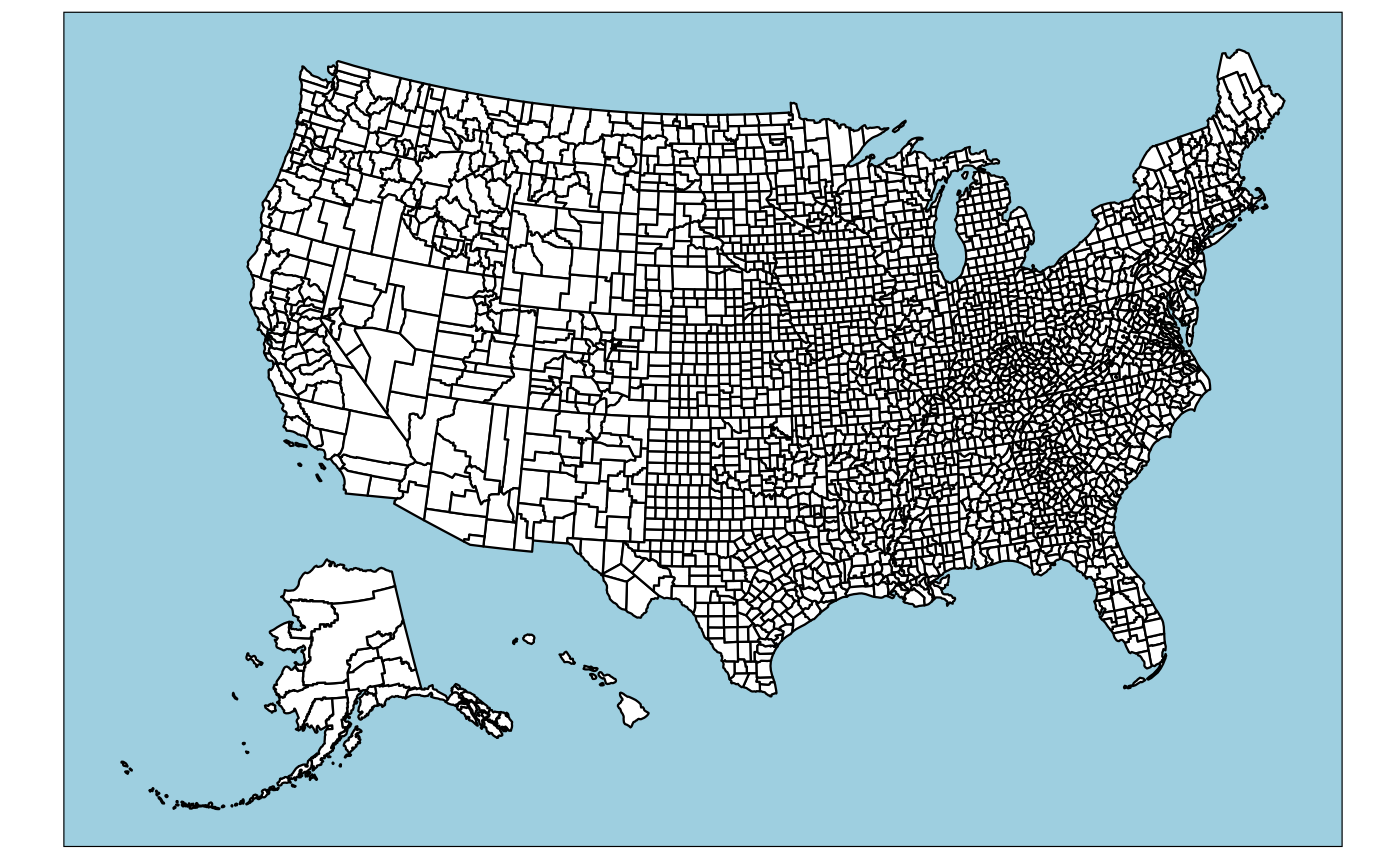
\includegraphics[width=\textwidth]{images/task1/U.S. counties.png}
    \end{minipage}%
    \begin{minipage}[c]{0.4\textwidth}
        \caption{Map of U.S. counties (Alaska and Hawaii have been displaced for a more compact representation)}
        \label{fig:us_counties}
    \end{minipage}
\end{figure}

The task is to build a network for each U.S. state, where the nodes represent counties, based on a dataset describing social connectivity between different regions~\cite{sciFacebook}. Each edge is characterized by a \textsl{Social Connectivity Index (sci)}.

This measure was first proposed and analyzed in~\cite{bai2018sci}.

Formally, the \textsl{sci} between two locations $i$ and $j$ is defined as:

\begin{equation}
    sci_{i,j} = \frac{\text{FB Connections}_{i,j}}{\text{FB Users}_i \times \text{FB Users}_j}
\end{equation}

where $\textsl{FB Users}_i$ and $\textsl{FB Users}_j$ are the numbers of Facebook users in locations $i$ and $j$, respectively, and $\textsl{FB Connections}_{i,j}$ is the total number of Facebook friendship connections between individuals in the two locations.

To protect individual privacy, the sci has been scaled between $1$ and $1,000,000,000$, with a small amount of noise added and the result rounded to the nearest integer.

The sci index can be interpreted as the \textbf{relative probability of a Facebook friendship} link between two users located in $i$ and $j$. In other words, if this measure is twice as large, a user in $i$ is twice as likely to be connected with a user in $j$.

The dataset provides edges, characterized by the columns: starting node ($\textbf{user\_loc}$), ending node ($\textbf{fr\_loc}$), and weight ($\textbf{scaled\_sci}$).

We consider the network as simple, ignoring friendships within each county.
% (Moreover, the network is undirected, since weights between the same pair of nodes are equal) 

\section{Data Handling}

For this analysis, we used the \textsl{igraph} package for network manipulation, \textsl{ggplot2} for plotting, and \textsl{tigris} for retrieving county information. Figure \ref{fig:us_counties} was generated using the \textsl{usmap} package.

The procedure was as follows: First, we imported a county dataset from \textsl{tigris} (from the year 2018 to match the county subdivisions in~\cite{bai2018sci}), modified it (for example, by adding a column for county centroids used later for plotting), and split it by state. Then, we imported the \textsl{US counties-US counties sci dataset} from~\cite{sciFacebook} and applied a similar procedure (removing edges between different states). Finally, we generated node and edge files for each state and plotted the corresponding networks.

Here is an example with California:

\begin{figure}[h]
    \centering
    \begin{minipage}[c]{0.6\textwidth}
        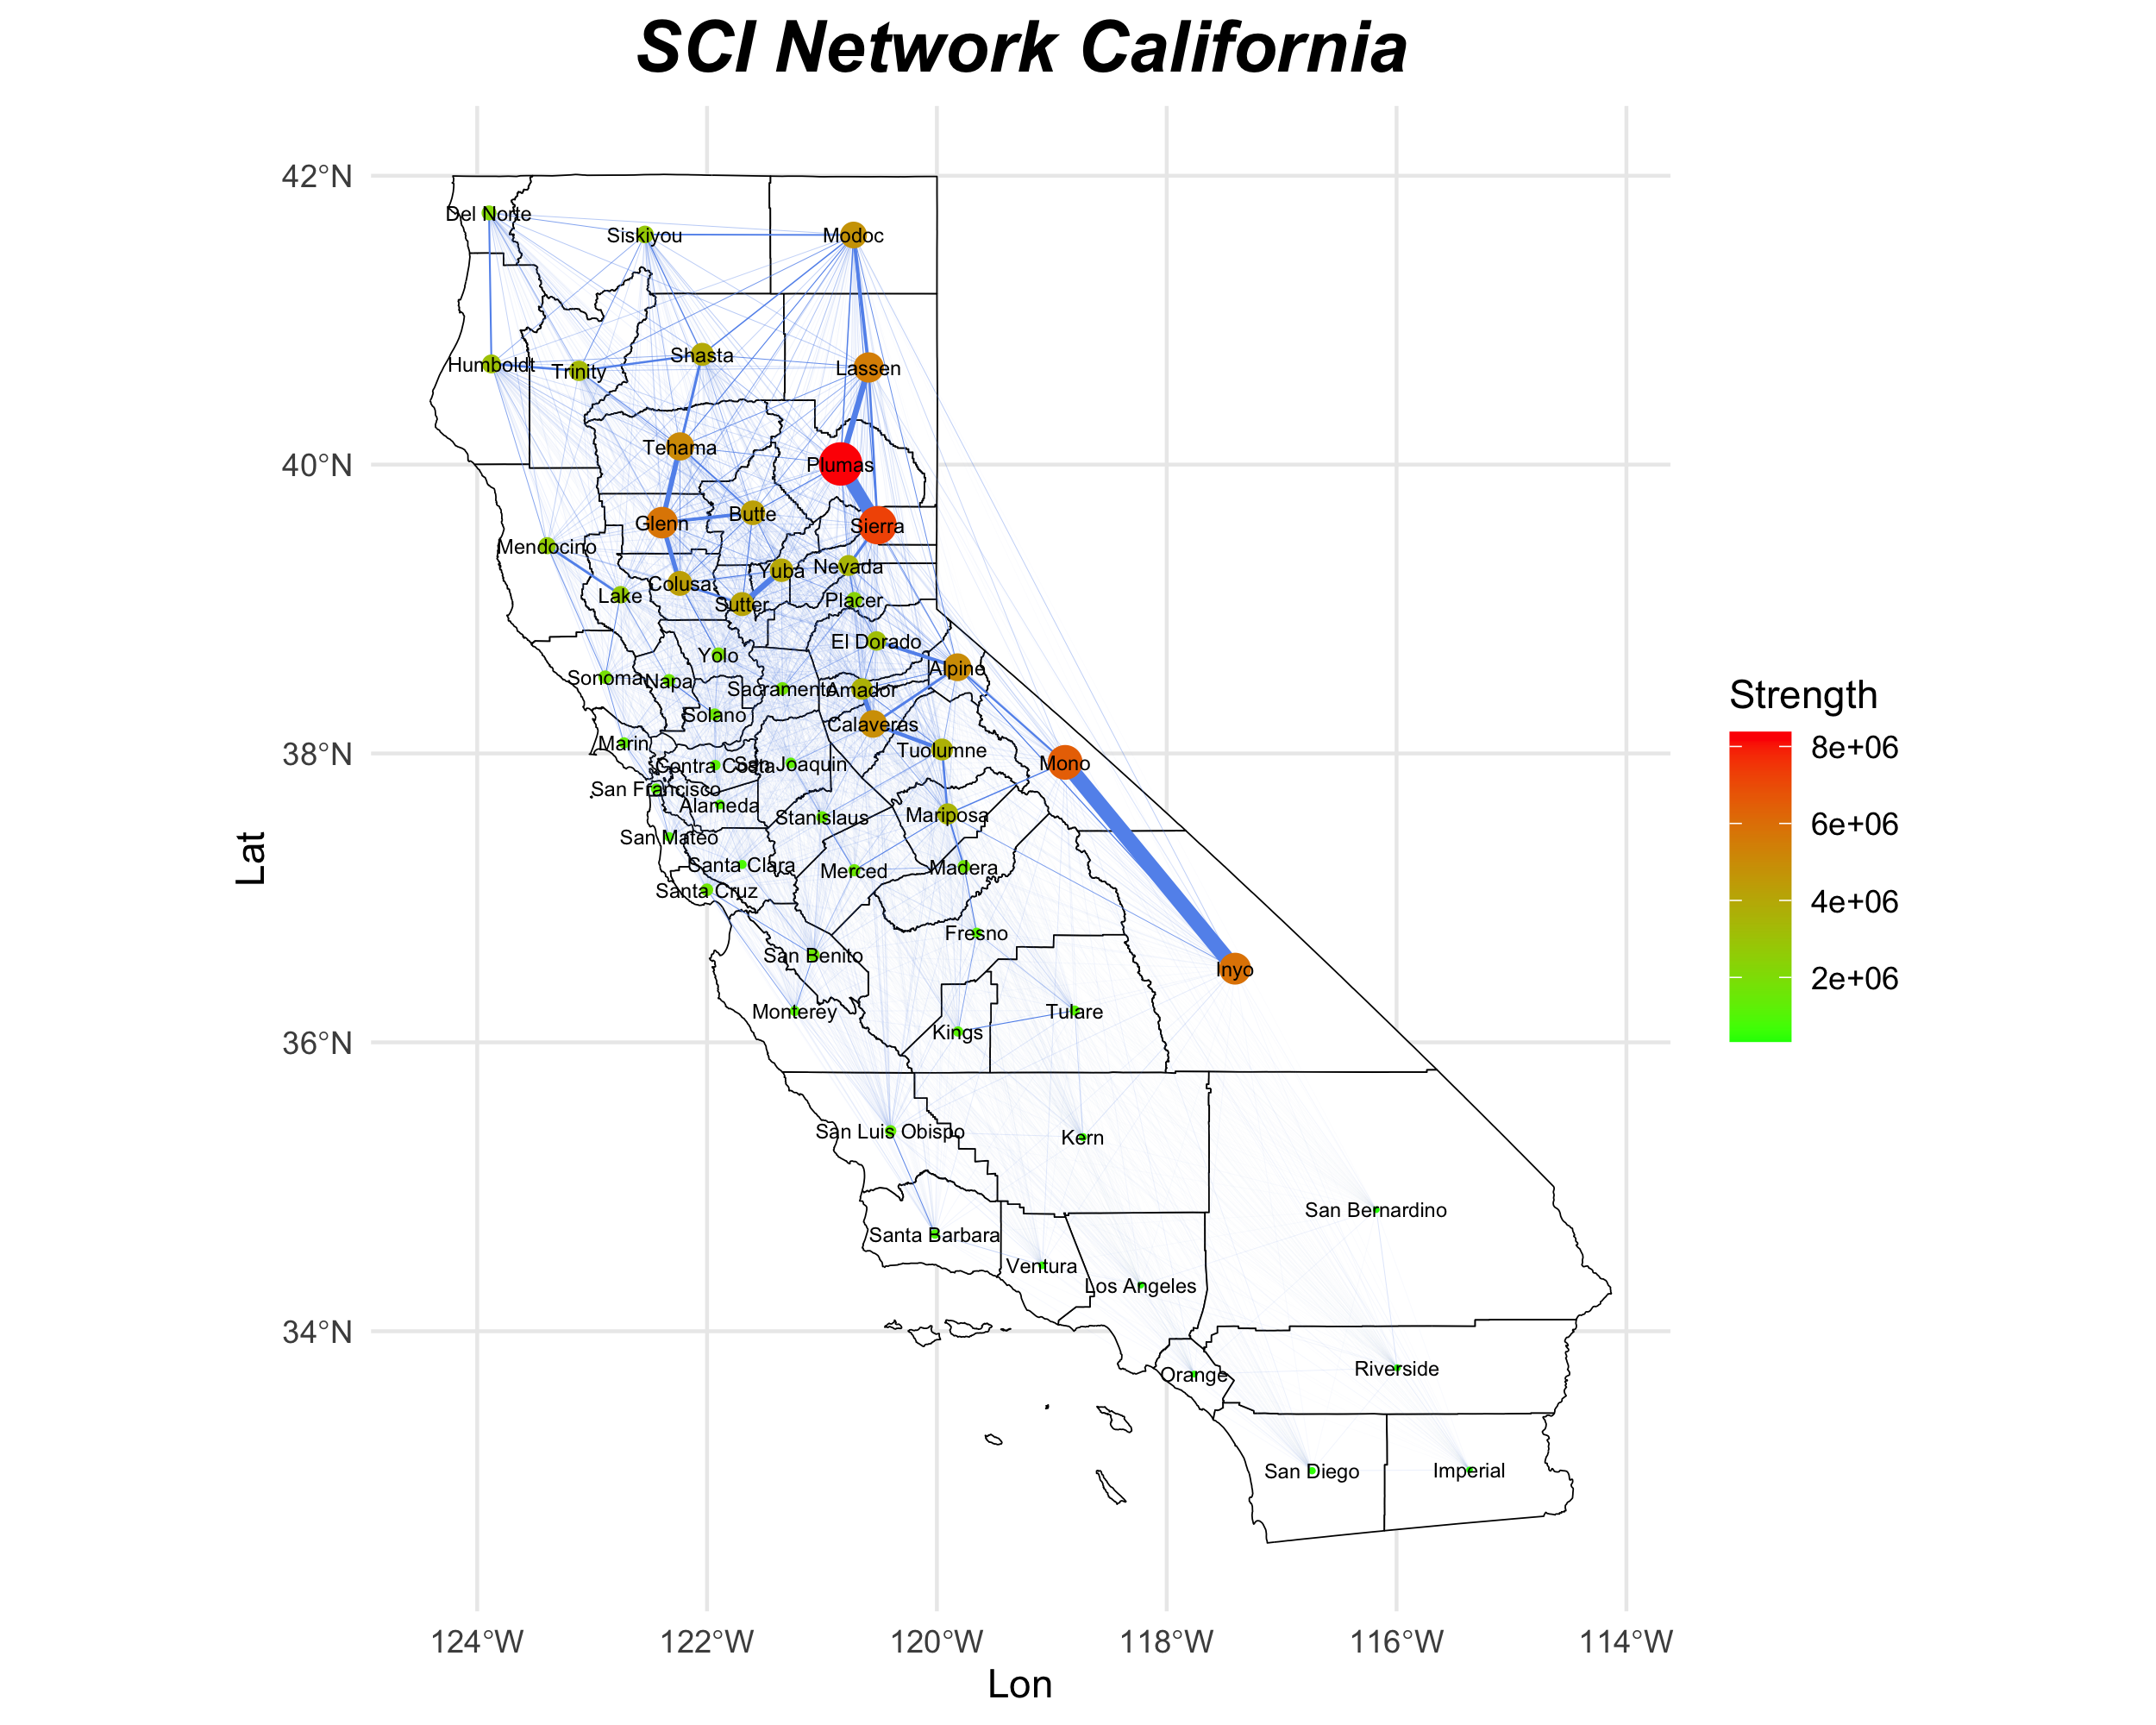
\includegraphics[width= \textwidth]{images/task1/California/network_California_strength.png} 
        \caption{California strength heatmap} 
    \end{minipage}%
    \begin{minipage}[c]{0.4\textwidth}
        \caption{California sci network (node size and color depend on its strength, and edge width is proportional to its weight)}
        \label{California:strength}
    \end{minipage}
\end{figure}

\begin{figure}[h]
    \centering
    \begin{minipage}[c]{0.7\textwidth}
        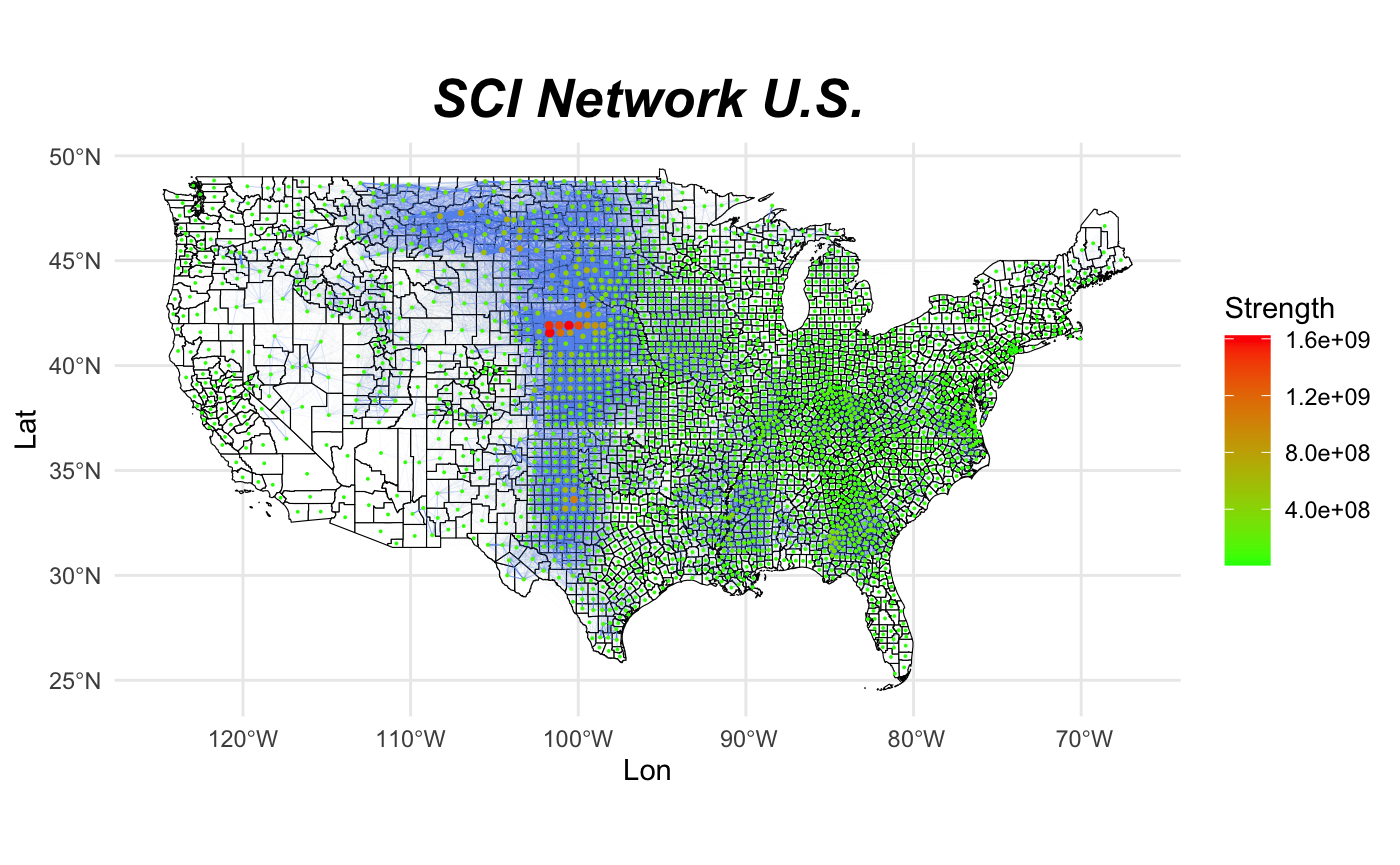
\includegraphics[width=\textwidth]{images/task1/U.S./US_network.png}
    \end{minipage}%
    \begin{minipage}[c]{0.4\textwidth}
        \caption{U.S. entire sci network (node size and color depend on its strength, and edge width is proportional to its weight)}
        \label{fig:us_counties}
    \end{minipage}
\end{figure}

\newpage

\section{Data Analytics}

Regions with only one node were excluded from the analysis. Even with this criterion, network sizes vary significantly, from the \textsl{U.S. Virgin Islands} with just 3 nodes, to \textsl{Texas} with 254 nodes (the average is around 60 nodes).

Most networks are complete, except for \textsl{American Samoa}, \textsl{Hawaii}, and the \textsl{Northern Mariana Islands}—each with 5 or fewer nodes—making degree analysis uninformative. Since the networks are weighted, we focused on node strength, as shown in figure \ref{California
}, and used SCI in the descriptors.

Interestingly, counties with the highest strength often have smaller populations. This may be because intra-county connections were ignored, and people in less populated areas tend to have more long-range friendships compared to those in denser regions.

We also generated histograms to analyze the strength distribution per state and across the U.S. While no clear patterns emerged from the frequency histograms, focusing on states with more than 100 counties (where statistical analysis is more reliable) reveals a consistent shape: an initial peak followed by a sharp decrease in frequency for higher strengths.

%add something on centrality


%bin=2*10e6
\begin{figure}[h]
\begin{minipage}[t]{0.4\linewidth}
\centering
\includegraphics[width=\textwidth, page=45]{images/task1/strenght_plots.pdf} 
%    \caption{Texas strength distribution}
    \label{Texas:strength}
\end{minipage}
\hfill
\begin{minipage}[t]{0.4\linewidth}
\includegraphics[width=\textwidth, page=48]{images/task1/strenght_plots.pdf} 
%    \caption{Texas strength distribution}
    \label{Virginia:strength}
\end{minipage}
%\end{figure} 


%\begin{figure}[h]
\begin{minipage}[t]{0.65\linewidth}
\centering
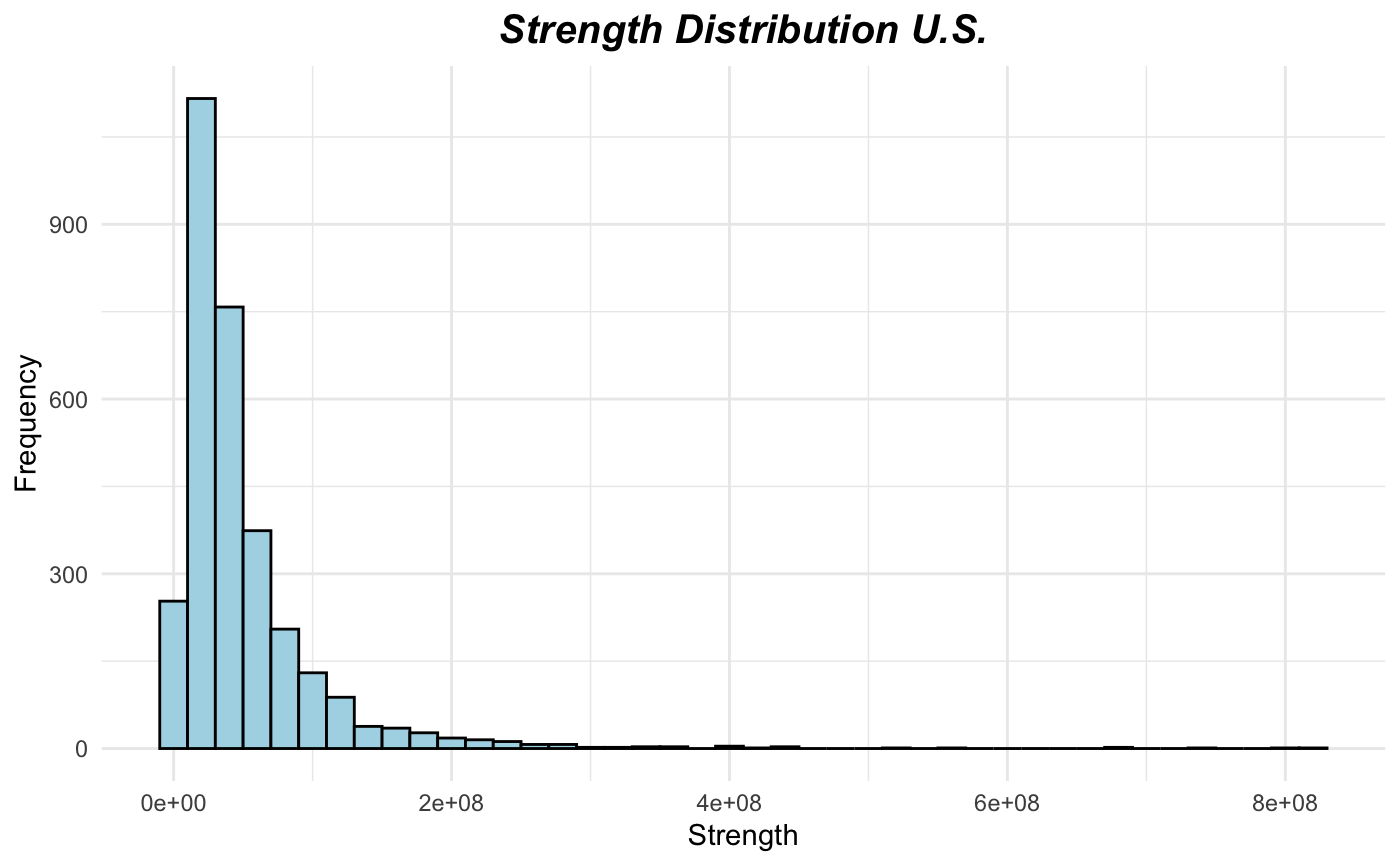
\includegraphics[width=\textwidth]{images/task1/U.S./strength_distibution_US.png} 
%    \caption{Texas strength distribution}
    \label{U.S.:strength}
\end{minipage}
\hfill
\begin{minipage}[t]{0.4\linewidth}
\includegraphics[width=\textwidth, page=17]{images/task1/strenght_plots.pdf} 
%    \caption{Texas strength distribution}
    \label{Virginia:strength}
\end{minipage}
\end{figure} 
%in this case uniform binning, binwidth=2*10e6


%differences across states: East-West ??
%add table of states and main descriptors ?


\chapter*{Remarks}
Part of the code was generated with the assistance of ChatGPT (v4), though never used blindly. For example, it suggested using the \textsl{tigris} package, helped build functions for degrees-DMS conversions, and provided a base layout for network and state map plotting. Additionally, this tool was helpful in checking grammar and making minor adjustments to improve the readability of this text.





